\section{Background and Related Work}
\label{sec:related_work}

\textbf{Polarization} has a long research history in computer vision and is widely used in many tasks such as reflection removal \cite{wieschollek2018separating, lei2020polarized, li2020reflection}, surface normal and/or shape estimation \cite{chen2017multi, kadambi2015polarized}, and semantic segmentation \cite{mei2022glass, kalra2020deep}. Light is an electromagnetic wave, with its electric field oscillating perpendicularly to the direction of propagation. Unpolarized light has a randomly fluctuating electric field while polarized light has a biased direction of the electric field. Common light sources like the sun and LED spotlights emit unpolarized light which would become partially/fully polarized light when passing through a linear polarizer, reflecting off certain materials, or undergoing certain types of scattering.

In this work, we focus on the linear polarization measurement captured by the off-the-shelf polarization-array CMOS sensor which can record light intensities in four polarization directions, \textit{i.e.}, $I_{0^{\circ}}$, $I_{45^{\circ}}$, $I_{90^{\circ}}$, and $I_{135^{\circ}}$, respectively. The polarization state of the light can be described using the Stokes vector $S=[S_0, S_1, S_2, S_3]$, where $S_0$ stands for the total light intensity, $S_1$ and $S_2$ describe the ratio of the $0^{\circ}/45^{\circ}$ linear polarization over its perpendicular counterpart, and $S_3$ is the circular polarization power. The Stokes elements $S_0, S_1, S_2$ are formally defined as:
\begin{align} 
\label{eq:stokes}
\begin{array}{lr}
    S_0 =I_{0^{\circ}} + I_{90^{\circ}} = I_{45^{\circ}} + I_{135^{\circ}},\\
    S_1 =I_{0^{\circ}}-I_{90^{\circ}},\\
    S_2 =I_{45^{\circ}}-I_{135^{\circ}}.
\end{array}
\end{align}

The angle of linear polarization (AoLP) $\phi$ and the degree of linear polarization (DoLP) $\rho$ are then be calculated via:
\begin{align} 
\label{eq:polar}
    \phi = \frac{1}{2}arctan(\frac{S_2}{S_1}), \quad \rho = \frac{\sqrt{S_1^2+S_2^2}}{S_0}.
\end{align}

As shown in Fig. \ref{fig:samples}, the trees, walls or sky in the background usually exhibit a low linear polarization degree while the glass, rubber and plastic parts of a car are typically with a high linear polarization degree. This observation inspires us to exploit the material cues revealed by polarization for robust car detection.

\begin{figure*}[ht]
    \centering
    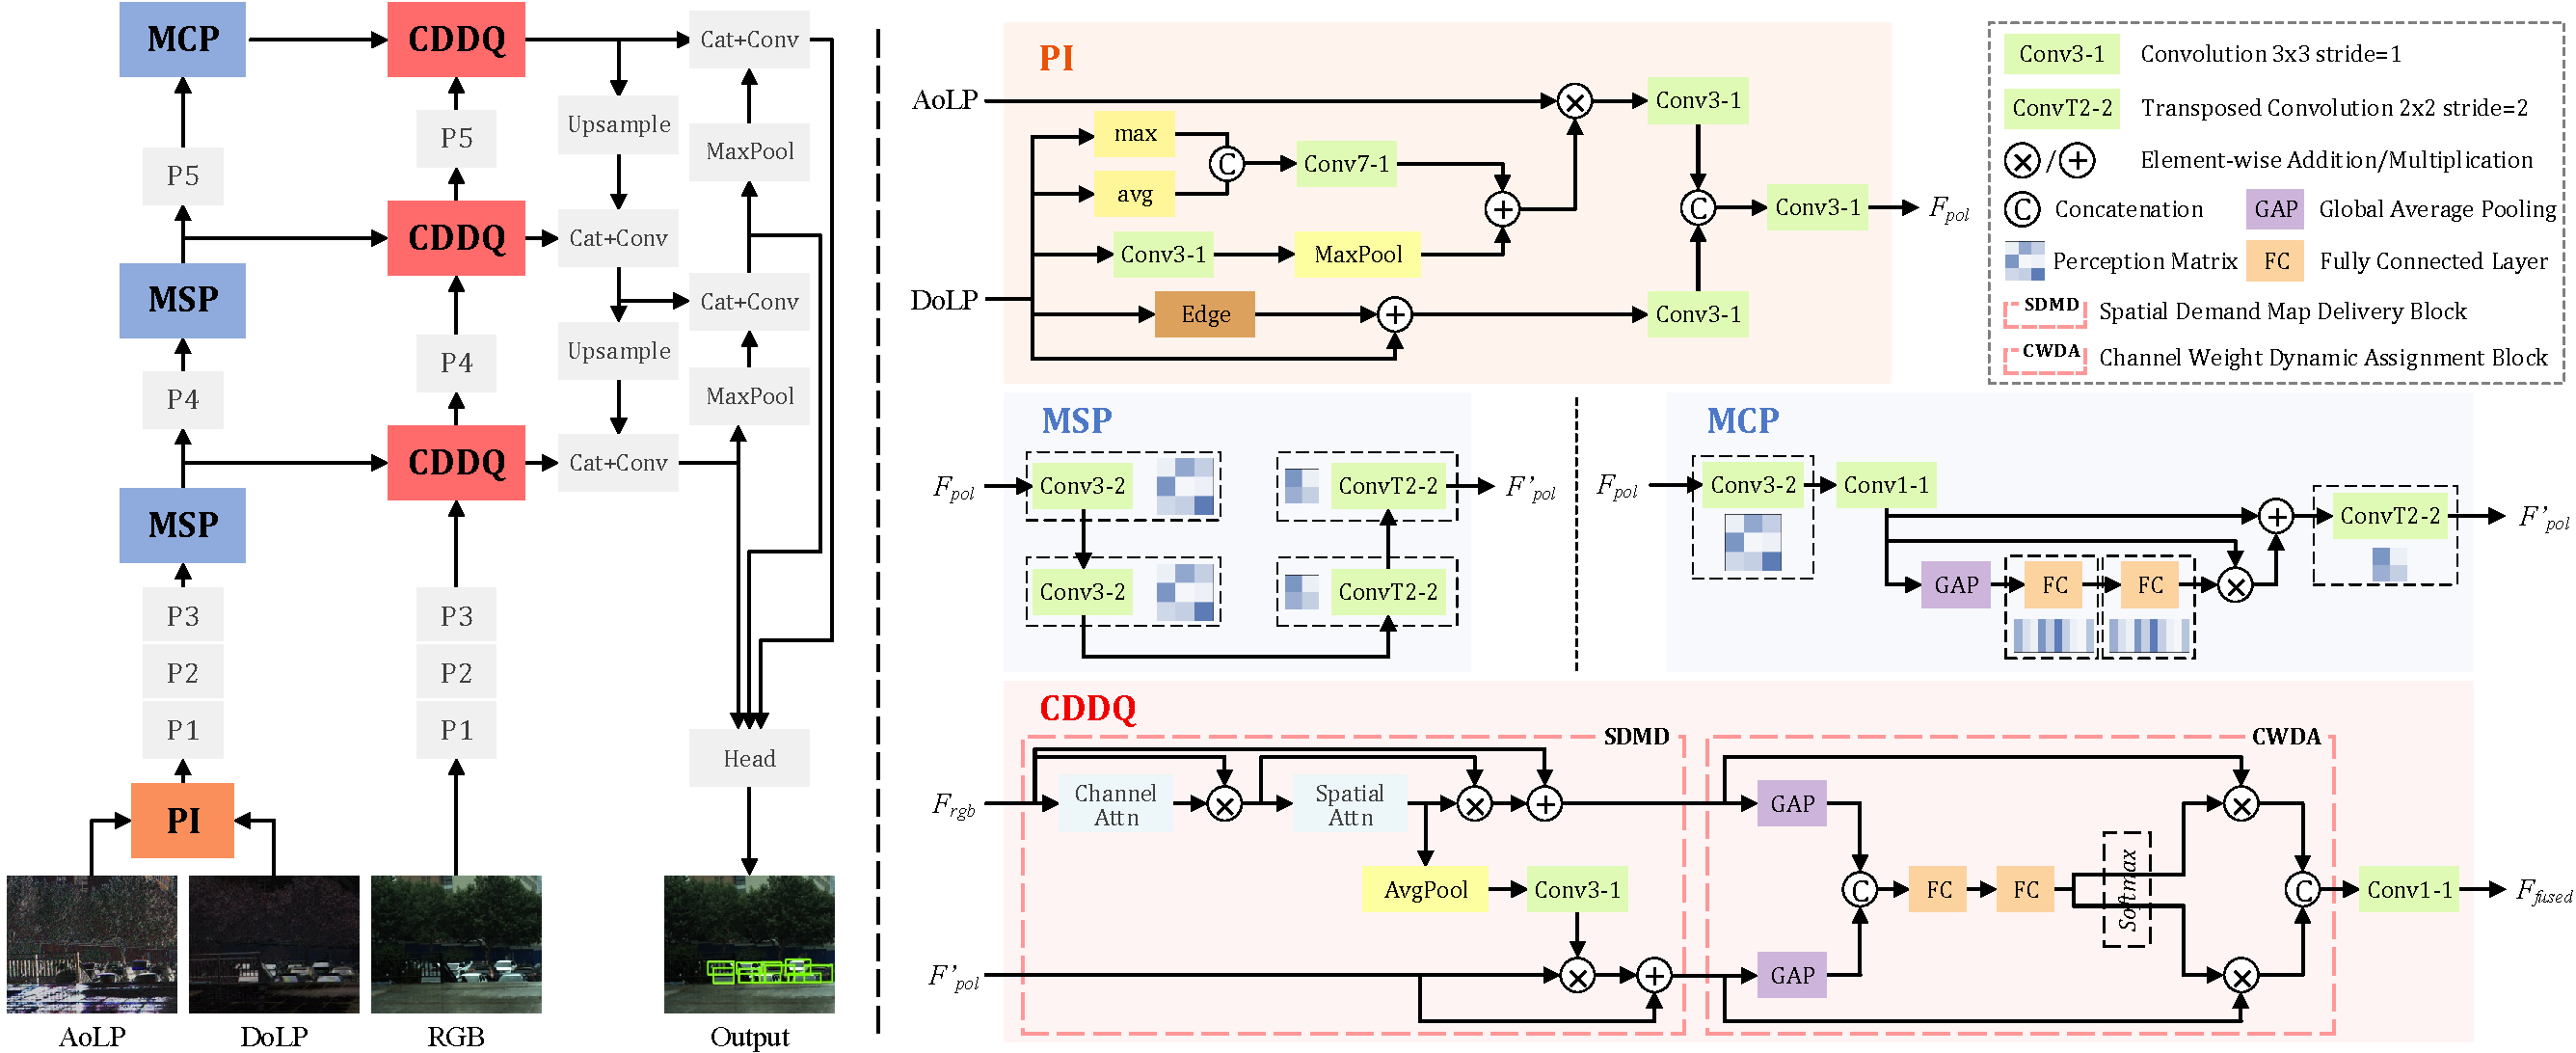
\includegraphics[width=\linewidth]{figure/methodology.pdf}
    \caption{Overview of PCDNet and its three main modules: the Polarization Integration (PI) module, the Material Spatial/Channel Perception (MSP/MCP) module, and the Cross Domain Demand Query (CDDQ) module.}
    \label{fig:pipeline}
\end{figure*}

\textbf{Object Detection} has achieved significant progress with the revolution of deep learning. Many state-of-the-art approaches emerged, including region-based detectors (\textit{e.g.}, Faster R-CNN \cite{Ren_2017} and EfficientDet \cite{tan2020efficientdet}), one-stage detectors (\textit{e.g.}, YOLO \cite{redmon2016you}, SSD \cite{liu2016ssd}, and RetinaNet \cite{lin2017focal}), and anchor-free detectors (\textit{e.g.}, FCOS \cite{tian2019fcos}). These methods typically employ advanced network architectures such as ResNet \cite{he2016deep}, VGG \cite{simonyan2014very} and EfficientNet \cite{tan2019efficientnet}. The trend in object detection has been toward the development of large models. The Vision Transformer \cite{dosovitskiy2020image}, derived from natural language processing \cite{zaheer2020big}, has achieved notable improvements in the field of object detection. For example, some methods such as Swin Transformer \cite{liu2021swin}, DETR \cite{carion2020end}, and DAB-DETR \cite{liu2022dabdetr} have achieved remarkable results on benchmark datasets including Microsoft COCO \cite{lin2014microsoft} and PASCAL VOC \cite{everingham2010pascal}. However, such models often exceed the hardware load and detection speed requirements of most restricted terminal devices. Moreover, most of them rely on clear and optimal RGB images which is hard to obtain in challenging scenes. Image enhancement and restoration on the low-quality RGB image will cost extra computing power and time. Our method differs from the above works in that we introduce reliable polarized material cues to complement traditional RGB features and design an RGB-P-based multimodal fusion network for robust detection.

\textbf{Multimodal Fusion} can provide rich contextual information for robust object detection \cite{valverde2021there, bijelic2020seeing}. Blin et al. employed a simple fusion method by stacking the multimodal data in the channel dimension to replace the original input \cite{blin2019road}. Manjunath et al. and Chen et al. adopted the concatenation \cite{manjunath2018radar} and element-wise addition \cite{chen2017multi} to fusing the low-level features of LiDAR and RGB, respectively. The attention mechanism \cite{vaswani2017attention} is also used to achieve multimodal fusion. HAFNet \cite{zhang2020hybrid} developed a cross-modal attention mechanism to perform feature fusion. Mei et al. calculated dynamic fusion weights for RGB and depth, considering the quality of each modality \cite{mei2021depth}. Similarly, Ji et al. used global average pooling followed by a fully connected layer to compute the channel attention weight for each modality \cite{ji2021calibrated}. Mei et al. generated spatial attention maps based on both global and local features to guide the multimodal fusion \cite{mei2022glass}. Although these methods achieve performance improvement to some extent, they perform information compensation in a passive ``post'' manner, resulting in the limited robustness of the model in challenging scenes. In this work, we develop a novel polarization material perception scheme to learn the intrinsic material properties of cars and a proactive multimodal fusion strategy to compensate RGB features with informative polarization cues in a ``request-and-complement'' manner, enhancing the robustness of car detection.
